\chapter{Transfer Function Optimization Using Visibility-Weighted Saliency \label{transfer_function_optimization}}
In this chapter, we present a transfer function optimization approach using the visibility-weighted saliency metric discussed in Chapter~\ref{visibility-weighted_saliency}.
This is an automated approach that adjusts transfer functions to match the visibility-weighted saliency towards user-specified targets.
In addition, a parallel line search strategy is presented for exploiting the computing power of multi-core processors to improve the performance of the transfer function optimization approach.

\section{Introduction}
Volume visualization is an effective means of discovering meaningful features in volume data sets.
Both exterior and interior of structures can be revealed simultaneously in a semi-transparent manner by specifying opacity values for the features in transfer functions \cite{wang_efficient_2011}.
Features could include intensity intervals in 1D transfer functions, rectangular or other shapes in 2D or higher-dimensional transfer functions.

In the specification of transfer functions for volume visualization, users often have a rough idea of how clear and opaque each feature should be and then adjust the opacity value of the features accordingly.
However, the relationship between the opacity of features and the saliency of the features in the final image is not linear.
The saliency of a feature in the final image depends on the opacity value assigned to the feature as well as the neighborhood of the feature and view-dependent occlusion of the feature.

%Therefore, it is desirable to have an automated method to assist the user in the design of transfer functions. In this chapter, we propose an optimization approach to automatically refine a user-defined transfer function towards target saliency levels specified by the user.

Therefore, it is desirable to have an automated method to assist the user in the design of transfer functions that match target saliency levels specified by the user. In this chapter, we propose an optimization approach that supports this requirement by automatically refining a user-defined transfer function towards any given saliency distribution.
Moreover, we present a parallel line search strategy to improve the performance of the transfer function optimization.

\section{Related Work}
% line search \cite{armijo_minimization_1966}
% conjugate gradient descent \cite{shewchuk_introduction_1994}
Transfer function specification is a non-trivial and unintuitive task in volume visualization. Compared to typical transfer function approaches, which are often subjective, it is desirable to have objective feedback regarding the clarity of features in volume visualization.

%Based on the perceptual principles, Chen et al. \cite{chan_perception-based_2009} introduced several image quality measures to enhance the perceived quality of semitransparent features.
%J{\"a}nicke and Chen \cite{janicke_salience-based_2010} described a quality metric for analyzing the saliency of visualization images and demonstrated its usefulness with examples from information visualization, volume visualization and flow visualization.

Correa and Ma \cite{correa_visibility-driven_2009} introduced visibility histograms to guide transfer function design for both manual and automatic adjustment.
Visibility histograms (Figure~\ref{fig:correa_visibility-driven_2009}), which summarize the distribution of visibility of voxels from a given viewpoint, are a powerful feedback mechanism for volume visualization \cite{emsenhuber_visibility_2008}.
Wang et al. \cite{wang_efficient_2011} extended visibility histograms to feature visibility histograms, in order to measures the influence of each feature to the resulting images. They described a scheme that allows users to specify a desired visibility for features of interest and subsequently the opacity transfer function is optimized using an active set algorithm \cite{polyak_conjugate_1969}.

%\noindent\makebox[\linewidth]{\rule{\paperwidth}{0.4pt}}

Researchers have developed a variety of parallel strategies to accelerate sequential optimization algorithms \cite{spedicato_algorithms_2012}.
%\cite{koko_parallel_1998}
Phua et al. \cite{phua_parallel_1998} proposed a parallel extension to quasi-Newton methods \cite{yang_optimization_2001}. Their approach generates several search directions at each iteration and then applies different line search and scaling strategies in parallel along each search direction.
Peachey et al. \cite{peachey_parallel_2009} presented another approach to parallelize the quasi-Newton methods.
In their applications, the objective function evaluation typically requires minutes or hours of processing time. Therefore, they introduced an approach that evaluates the objective function in parallel over a cluster of computers and continues to the next iteration before all evaluations finish in order to accelerate convergence.

%-------------------------------------------------------------------------
\section{Method}
In Chapter~\ref{visibility-weighted_saliency}, visibility-weighted saliency was proposed as a measure of visual saliency of features in volume visualization. This metric indicates the perceptual importance of voxels and the visibility of features in volume rendered images and can be utilized to assist users in choosing suitable viewpoints and designing effective transfer functions to visualize the features of interest.
In this chapter, we describe a transfer function optimization approach based on the visibility-weighted saliency metric in order to automatically adjust the volume visualization to satisfy user-specified targets set on the visibility-weighted saliency for the features.

The approach described in Chapter~\ref{transfer_function_refinement} is an automated method of optimizing transfer functions, based on the intensity distribution of voxels in the volume data set. However, this approach does not take into account the spatial distribution of voxels and the viewpoint of the visualization. Visibility-weighted saliency, on the other hand, takes into account both of these two aspects. The visibility-weighted saliency consists of two component fields, i.e. saliency field and visiblity fields. Saliency fields are essentially difference of Gaussians, which include the information of local neighborhoods of voxels.
Visibility fields are computed from opacity contribution of voxels to volume rendered images, which indicate viewpoint dependent occlusions of the voxels.

Constraints are introduced in the search of the parameter space. Only the opacity of features are changed in the transfer function domain. The definition of features (e.g. intensity ranges on 1D transfer functions) and the colors of features remain the same.
%done the classification of features.
These constraints are based on the assumption that the user has explored the volume data and done the classification of features.
% set up the transfer function according to his/her needs.
Our approach aims to help the user adjust the saliency distribution and reduce occlusion while preserving the user's knowledge or judgments of the data set.
While the approach discussed in Chapter~\ref{transfer_function_refinement} was designed for exploration and visual search of volume data, the approach in this chapter could aid in analysis, understanding or closer inspection of the data.

%Should maybe say here and/or in the conclusions that (while Ch3 was for exploring, visual search of data) the contributions of this chapter could aid in analysis, understanding or closer inspection of the data

\subsection{Objective Function}
Users define target importance values for each feature in the transfer function domain.
Our transfer function optimizer adjusts the transfer function to match the visibility-weighted saliency with the user-defined target saliency values.
Multiple saliency fields computed from different appearance attributes can be combined together in order to represent different aspects of the visual saliency of voxels.
In our implementation, brightness and saturation are used respectively to compute visibility-weighted saliency fields and define the weighted sum of the two sets of feature saliency as visibility-weighted feature saliency.
The objective function $ F $ is defined as the root mean square of the differences of the visibility-weighted saliency and target importance of each feature.
\[ F=\sqrt{ \frac{\sum_{i=1}^{n} (W_{i}-t_{i})^{2}}{n} } 
\addtag \]
where $ W_{F}=u_{1}W_{F}(O_{b},i,\sigma)+u_{2}W_{F}(O_{s},i,\sigma) $ is the visibility-weighted saliency of feature $ i $, and $ t_{i} $ is the user-defined importance of feature $ i $. These user-defined saliency values are normalized and they add up to 1, in other words, $ t_{i} \in [0.1] $ and $ \sum_{i=1}^{n} t_{i} = 1 $.

As previously described in Section~\ref{weighted_feature_saliency}, multiple saliency fields computed from different appearance attributes can be combined together in order to represent different aspects of the visual saliency of voxels.
In our implementation, $ W_{F}=u_{1}W_{F}(O_{b},i,\sigma)+u_{2}W_{F}(O_{s},i,\sigma) $ is a weighted sum of visibility-weighted saliency values computed using brightness and saturation of voxels respectively, and $ u_{1} $ and $ u_{2} $ are weights of the two appearance attributes.

However, the visibility-weighted saliency $ W_{i} $ is not a variable that can be directly modified. Instead, $ W_{i} $ is a complicated function of the color and opacity of voxels in feature $ i $ and is also influenced by the viewpoint of rendering. A visibility-weighted saliency field is a combination of a visibility field and a saliency field. The saliency field is a view-independent field based on the color of every voxel in the volume data set, while the visibility field is a view-dependent field computed from the opacity contribution of every voxel to the final image when rendered from a certain viewpoint.

The computation of visibility fields is non-trivial. In order to compute a visibility field, a slice-based rendering is performed on a series of quads which are parallel to the viewing plane, one for each slice.
Subsequently, the visibility values are computed by subtracting the accumulated opacity of the previous slice from that of the current slice. After collecting the visibility values of all voxels, the visibility field can be constructed. The details of visibility fields were previously described in Section~\ref{visibility_fields}.

The evaluation of the objective function is computationally expensive. However, in an iterative optimization, the visibility field and visibility-weighted saliency have to be recomputed at each step after the feature opacity values are updated.

\subsection{Parameter Space}
We use a nucleon data set \cite{website:Voreen_datasets_2013} to demonstrate how the visibility-weighted saliency of features change when the feature opacity values change. As displayed in Figure~\ref{fig:nucleon_naive}, three features are defined in the transfer function for the nucleon data set.

The dimension of the parameter space is the same as the number of features defined by the user. In this case, three features are defined for the nucleon data set. The opacity of each feature is mapped to an axis in the parameter space. Therefore, the opacity values of the 3 features are mapped to $ x, y, z $ axes of a 3D scalar field respectively.
%Figure~\ref{fig:nucleon_densityplot} displays three 3D scalar fields, one for each feature, to provide an intuitive overview of the relationship between the feature opacity values and the visibility-weighted saliency values.
Figure~\ref{fig:nucleon_densityplot} displays a visualization of three 3D scalar fields representing this parameter space.
One field is presented for each feature to provide an intuitive overview of the relationship between the feature opacity values and the visibility-weighted saliency values. In order to avoid confusion, please note that this has no spatial relationship to the actual 3D volume data (which is itself a 3D scalar field).
%I suggest saying something like; Figure 5.2 displays a visualization of three 3D scalar fields representing this parameter space. One field is presented for each feature to provide an intuitive overview of ....  . In order to avoid confusion, please note that  this has no spatial relationship to the actual 3D volume data (which is itself a 3D scalar field).

Feature 1 (the purple structure in Figure~\ref{fig:nucleon_naive}) is the exterior of the nucleon data set, the visibility-weighted saliency of this feature is shown in the 3D scalar fields in the same color at the left in Figure~\ref{fig:nucleon_densityplot}.
The visibility-weighted saliency of Feature 1 increases as its opacity increases,
%as shown in the 3D scalar fields that the brightness and opacity increase along $ x $ axis.
as demonstrated by the fact that both the brightness and opacity of the corresponding 3D field increases along the $x$-axis.
Similar patterns also appear in the other 2 scalar fields, the visibility-weighted saliencies of Feature 2 (the red structure in Figure~\ref{fig:nucleon_naive}) and Feature 3 (the green structure in Figure~\ref{fig:nucleon_naive}) also increase as their opacity values increase.

%I Suggest: ", as demonstrated by the fact that both the brightness and opacity of the corresponding 3D field increases along the x-axis."

%Thus it is reasonable to assume that the visibility-weighted saliency of a feature is a monotonic function of its opacity.

Moreover, Feature 1 is the exterior of the nucleon, its visibility-weighted saliency is almost not influenced by the opacity of other features. On the other hand, the visibility-weighted saliency of Feature 2 is influenced by both the opacity of Feature 1 and Feature 2. In addition, the visibility-weighted saliency of Feature 3 is drastically influenced by the opacity of Feature 1, Feature 2 and Feature 3, as Feature 3 is an interior structure and can be easily occluded by the other 2 features.

In order to demonstrate the distribution of the objective function in the parameter space $ x \in [0,1] $, $ y \in [0,1] $ and $ z \in [0,1] $, we sample the parameter space with sampling interval $ 0.1 $, from 0 to 1 along each axis. There are 11 sampling points along each axis, which results in 1331 sampling points in the parameter space. In Figure~\ref{fig:nucleon_parameterspace}, the parameter space is rendered as a density plot with a color function resembling a temperate map which gradually changes from orange to blue.

\begin{figure}
\centering
\begin{minipage}{.3\textwidth}
	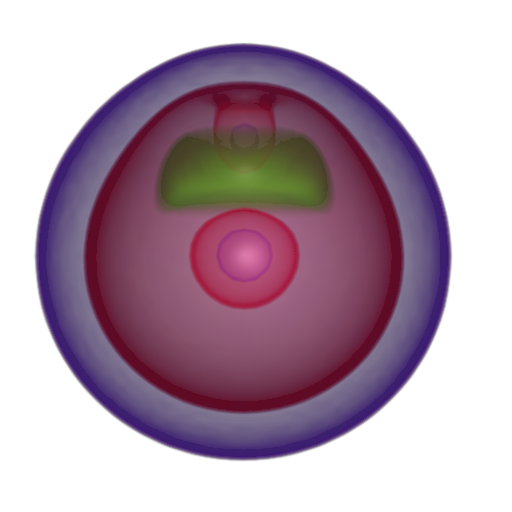
\includegraphics[width=1\linewidth]{images/nucleon_naive}
	\subcaption{}
\end{minipage}~
\begin{minipage}{.15\textwidth}
	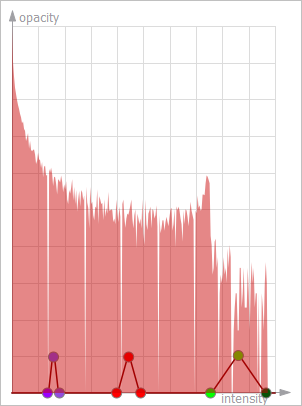
\includegraphics[width=1\linewidth]{images/tf_nucleon_naive}
	\subcaption{}
\end{minipage}~
\begin{minipage}{.25\textwidth}
	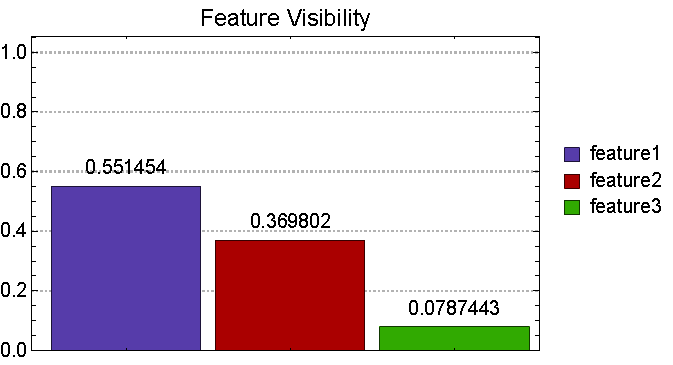
\includegraphics[width=1\linewidth]{figures/nucleon_naive_visibility_chart}
	\subcaption{}
\end{minipage}~
\begin{minipage}{.25\textwidth}
	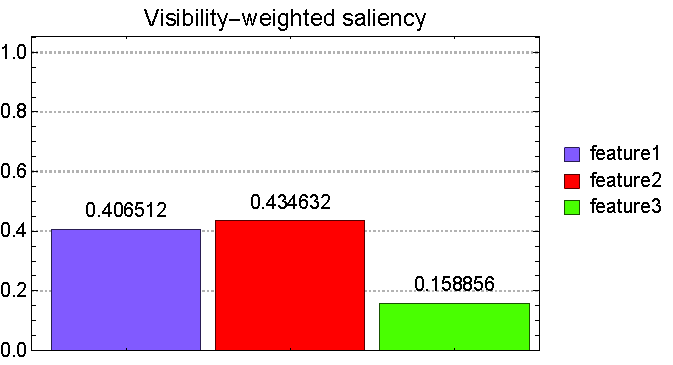
\includegraphics[width=1\linewidth]{figures/nucleon_naive_visibility_saliency_weighted_chart}
	\subcaption{}
\end{minipage}
\caption[A nucleon data set with a naive transfer function]{(a) A nucleon data set \cite{website:Voreen_datasets_2013}; (b) A naive transfer function with equal opacitity values for each feature; (c) The feature visibility histogram \cite{wang_efficient_2011}; (d) The visibility-weighted saliency histogram}
\label{fig:nucleon_naive}
\end{figure}

\begin{figure}
	\centering
	\begin{minipage}{.3\textwidth}
		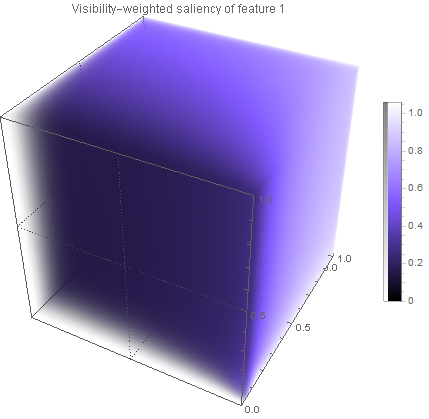
\includegraphics[width=1\linewidth]{images/nucleon_strong_red_densityplot1}
		\subcaption{}
	\end{minipage}~
	\begin{minipage}{.3\textwidth}
		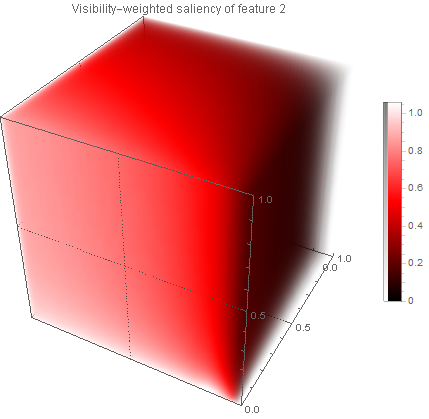
\includegraphics[width=1\linewidth]{images/nucleon_strong_red_densityplot2}
		\subcaption{}
	\end{minipage}
	\begin{minipage}{.3\textwidth}
		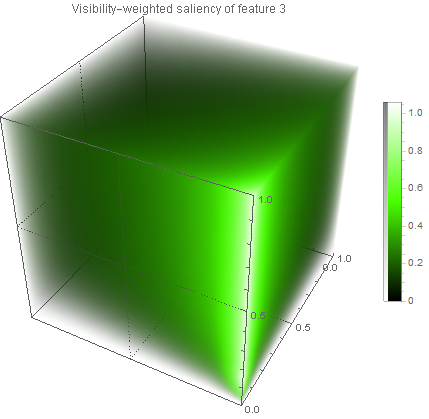
\includegraphics[width=1\linewidth]{images/nucleon_strong_red_densityplot3}
		\subcaption{}
	\end{minipage}
	\caption[Visibility-weighted saliency of the 3 features are mapped to brightness and opacity respectively.]{Visibility-weighted saliency of the 3 features are mapped to brightness and opacity of the 3D fields in (a), (b) and (c) respectively. The visibility-weighted saliency of Feature 2 (red) is affected by both the opacity of Feature 1 (purple) and Feature 2. The visibility-weighted saliency of Feature 3 (green) is affected by the opacity of Feature 1, Feature 2 and Feature 3.}
	\label{fig:nucleon_densityplot}
\end{figure}

\begin{figure}
	\centering
	\begin{minipage}{.6\textwidth}
		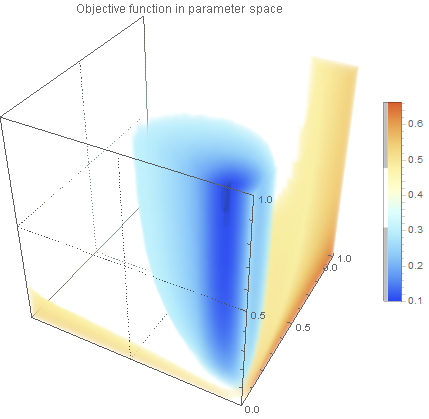
\includegraphics[width=1\linewidth]{images/nucleon_strong_red_parameterspace}
	\end{minipage}
	\caption[Each position (x, y, z) in the parameter space represents 3 features with opacity values (x, y, z).]{Each position (x, y, z) in the parameter space represents 3 features with opacity values (x, y, z). The value of the objective function (with \{0.1, 0.3, 0.6\} as target) is mapped to the color in the parameter space (with sampling interval $ 0.1 $). For clarity, only the high and low values are visible and the data range in the middle is set to transparent.}
	\label{fig:nucleon_parameterspace}
\end{figure}

\subsection{Optimization Algorithm}
The gradient descent algorithm is employed in our transfer function optimizer.
Gradient descent is a first-order optimization algorithm. It is based on the observation that if a function $ f(x) $ is defined and differentiable in a neighborhood of a point $ x_{1} $, then $ f(x) $ decreases fastest in the direction of the negative gradient of the function \cite{chong_introduction_2013}.

Given a continuously differentiable function $ f(x) $ with $ x \in \mathbb{R}^{n} $, let $ x_{k} $ be the current iteration point and $ g_{k}=g(x_{k})= \nabla f(x_{k}) $ be the gradient of $ f(x) $ at $ x_{k} $. The gradient descent method defines the next iteration point by
\[ x_{k+1}=x_{k}- \alpha_{k} g_{k} , k \geq 0 \]
for $ \alpha_{k} $ small enough, then $ f(x_{k+1}) \leq f(x_{k}) $. The gradient varies as the iteration proceeds, tending to zero as it approaches a local minimum. When the gradient decreases, the iteration step sizes also decrease. So hopefully the sequence $ {x_{k}} $ converges to the desired local minimum after performing the iteration.

In gradient descent methods, we can either take very small step sizes and reevaluate the gradient at every step, or take large steps each time. If the step size is too small, it may end up in a laborious situation that the objective function converges very slowly. If the step size is too large, it results in a more zigzag path and may have the risk of missing the local minimum and thus cannot converge.

\subsection{Estimating Descent Directions \label{estimating_descent_directions}}
In each step of the optimization, the descent direction $ g_{k} $ has to be updated. 
As previously discussed, the visibility-weighted saliency of a feature increases as its feature opacity increases. 
%The visibility-weighted saliency of a feature is a monotonic function of the opacity of the feature. 
However, the relationship between the visibility-weighted saliency and the opacity of a feature also depends on the viewpoint of rendering and the spatial distribution of voxels of every feature in the volume data set. An exact derivative of the visibility-weighted saliency with respect to the opacity of the feature cannot be determined in advance.

In the following subsections, two methods for estimating descent directions are described.

\subsubsection{Gradients with Backward Difference}
The partial derivative of the objective function $ F $ with respect to $ x_{i} $ is
\[ \frac{\partial F}{\partial x_{i}} = \frac{\partial F}{\partial W_{i}} \frac{\partial W_{i}}{\partial x_{i}} \]
where $ x_{i} $ is the opacity and $ W_{i} $ is the visibility-weighted saliency of feature $ i $.
The partial derivative $ \frac{\partial F}{\partial W_{i}} $ can be solved from the objective function $ F $.
However, $ \frac{\partial W_{i}}{\partial x_{i}} $ cannot be determined without knowledge of the actual volume data set.

For a function $ f(x) $, its first-order derivative can be estimated by a backward difference divided by a small step.
\[ \frac{\nabla_{d}[f](x)}{d}=\frac{f(x)-f(x-d)}{d} \]
where $ d $ is a nonzero number.
When $ d $ is small, the backward difference divided by $ d $ approximates the derivative. Assuming that $ f $ is differentiable, the error in this approximation can be derived from Taylor's theorem.
\[ \frac{\nabla_{d}[f](x)}{d}-f'(x)=\mathcal{O}(d) \to 0 , \; as \; d \to 0 \]

The backward difference is used here to approximate $ \frac{\partial W_{i}}{\partial x_{i}} $, hence we have
\[ \frac{\partial W_{i}}{\partial x_{i}} \approx \frac{\nabla_{d}[W_{i}](x_{i})}{d} \]

The evaluation of the objective function $ F $ is very computationally expensive. In our implementation, a small step size $ d $ is adopted, therefore the backward difference can be calculated from values of the objective function, visibility-weighted saliency and steps of the previous iteration. In this case, no extra evaluation of the visibility-weighted saliency and the objective function is required.
%Similarly, the backward difference can calculated from previous values of the visibility-weighted saliency and step positions.

Furthermore, if the function $ W_{i} $ of $ x_{i} $ is approximately a linear function, the partial derivative $ \frac{\partial W_{i}}{\partial x_{i}} $ becomes constant and could be replaced by an empirical constant $ b_{i} $. In this case, the gradient of the objective function with respect to the visibility-weighted saliency is used instead, which should be more computationally efficient.
\[ \frac{\partial F}{\partial x_{i}} \approx \frac{\partial F}{\partial W_{i}} b_{i} \]

\subsubsection{Descent Directions with Second-Order Derivatives}
Newton's method, which is an iterative method for finding the roots of a differentiable function, can be used to find a minimum or maximum of a function. Because the derivative is zero at a minimum or maximum, minima and maxima can be found by applying Newton's method to the derivative.
\[ x_{k+1}=x_{k}- \frac{f'(x_{k})}{f''(x_{k})} \]
This iteration equation gives a similar form of gradient descent, thus $ \frac{\partial^2 F}{\partial x_{i}^2} $ can be adopted in our optimization algorithm as the descent direction.

The first-order derivative can be estimated by backward difference of the objective function $ F $, and the second-order derivative $ F'' $ can be estimated by backward difference of the first-order derivative $ F' $.
\[ \frac{\partial^2 F}{\partial x_{i}^2} 
\approx \dfrac{ \frac{\nabla_{d}[F](x_{i})}{d} }{ \frac{\nabla_{d}[F'](x_{i})}{d} }
= \frac{ \nabla_{d}[F](x_{i}) }{ \nabla_{d}[F'](x_{i}) } \]

\subsubsection{Comparison of Descent Directions}
We have tested the descent directions discussed above with several volume data sets with various step sizes.
All the above described methods worked with small step sizes. As the step size increases, using $ \frac{\partial F}{\partial W_{i}} \frac{\nabla_{d}[W_{i}](x_{i})}{d} $ as descent directions would be unstable. While using $ \frac{\partial F}{\partial W_{i}} b_{i} $ and $ \frac{ \nabla_{d}[F](x_{i}) }{ \nabla_{d}[F'](x_{i}) } $ as descent directions would be still stable even when the step sizes are large. In our implementation, $ b_{i}=1 $ is used and this yields desirable results.

Gradient descent was performed on several volume data sets with various transfer functions, using the two normalized descent directions computed from $ [ \frac{\partial F}{\partial W_{1}} b_{1} ... \frac{\partial F}{\partial W_{n}} b_{n} ] $ (Method 1)
 and 
$ [ \frac{ \nabla_{d}[F](x_{1}) }{ \nabla_{d}[F'](x_{1}) }  ... \frac{ \nabla_{d}[F](x_{n}) }{ \nabla_{d}[F'](x_{n}) } ] $ (Method 2).
In these preliminary results (Figure~\ref{fig:nucleon_naive_tooth_naive_rms}), the convergence speeds of the two methods were similar, with Method 2 slightly faster in some cases.

\begin{figure}
	\centering
	\begin{minipage}{.49\textwidth}
		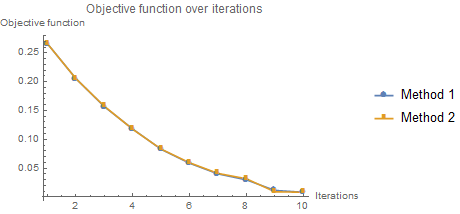
\includegraphics[width=1\linewidth]{images/nucleon_naive_rms_fixed_newton}
		\subcaption{}
	\end{minipage}~
	\begin{minipage}{.49\textwidth}
		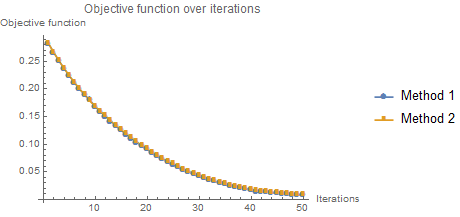
\includegraphics[width=1\linewidth]{images/tooth_naive_rms_fixed_newton}
		\subcaption{}	
	\end{minipage}
	\begin{minipage}{.49\textwidth}
		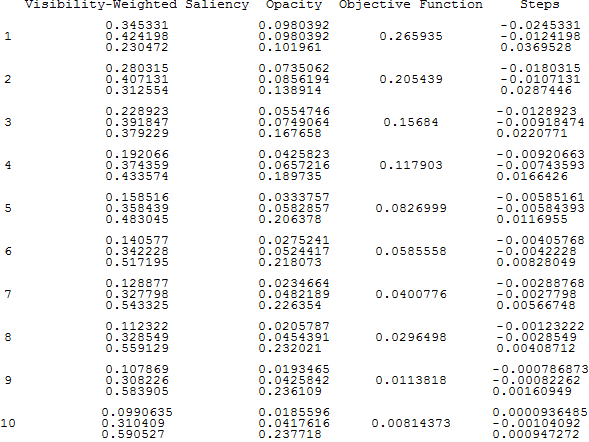
\includegraphics[width=1\linewidth]{images/nucleon_naive_table_fixed}
		\subcaption{}	
	\end{minipage}~
	\begin{minipage}{.49\textwidth}
		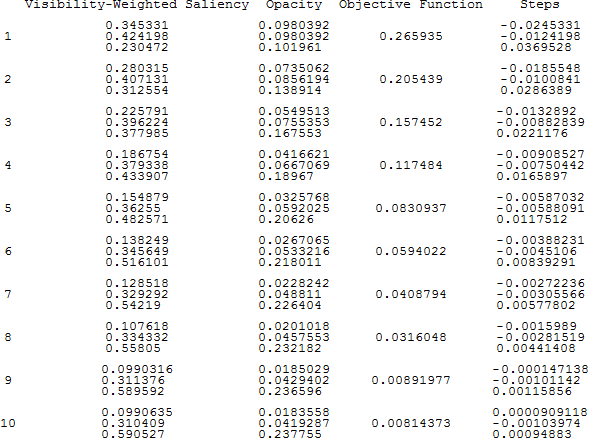
\includegraphics[width=1\linewidth]{images/nucleon_naive_table_newton}
		\subcaption{}	
	\end{minipage}
	\caption[The two methods for estimating descent directions are applied to transfer function optimization on the nucleon data set and a tooth data set]{The two methods for estimating descent directions are applied to transfer function optimization on the nucleon data set (a) and a tooth data set (b).
		Method 1 converges ($F<0.03$) at step 10 (as in the iteration log (c)) and method 2 converges at step 9 (as in the iteration log (d)) on the nucleon data set with a naive transfer function (assigning equal opacity to each feature).
		The two methods both converge at step 47 on the tooth data set with a native transfer function.}
	\label{fig:nucleon_naive_tooth_naive_rms}
\end{figure}

\subsection{Adaptive Step Size with Line Search}
Performing gradient descent with a small step size may result in converging too slowly and require a lot of evaluations of the objective function, which is rather expensive to compute in our situation. Various approaches have been proposed regarding the choices of step sizes, which lead to various gradient algorithms \cite{yuan_step-sizes_2008}.

\subsubsection{Line Search}
The line search strategy is an iterative approach that adapts the step size in gradient descent in order to achieve a reduction in the objective function while still making sufficiently fast progress.
\[ h( \gamma)=f(x_{k}+\gamma g_{k}) \]
where $ g_{k} $ is the descent direction and $ x_{k} $ is the current point at the $ k$-$th $ iteration.

There are two type of approaches of line search, exact line search and inexact line search \cite{vrahatis_class_2000}.
Exact line search chooses the next iteration point by achieving the least objective function value. However, despite the optimal properties, exact line search often behaves poorly and tends to zigzag in two orthogonal directions, which usually implies deteriorations in convergence \cite{zhou_gradient_2006}.
In contrast, inexact line search only loosely finds a sufficient decrease of the objective function along the descent direction.

The inexact line search we used in our implementation is as follows.

\begin{enumerate}
	\item Set initial iteration count $ i=0 $ and set $ n $ to the maximum iteration count.
	\item Check whether $ f(x_{k}+\gamma_{i+1} g_{k}) < f(x_{k}+\gamma_{i} g_{k}) $ where $ \gamma_{i}=2^{i} $
	\item If so and $ i<n-1 $, $ i=i+1 $ and repeat Line 2, otherwise terminate the line search.
\end{enumerate}

The step size $ \gamma_{n} $ is chosen after the above line search procedure.
This strategy does not find the exact minimum along the line direction, instead it yields reasonable results and descends much faster than using fixed step sizes.

With line search approaches, the optimization algorithm can converge much faster than using fixed step sizes. Figure~\ref{fig:nucleon_parameterspace_path} displays the paths of two gradient descent methods, one progresses regularly with fixed step sizes, the other progresses aggressively with line search. It takes fewer steps for the latter to reach a local minimum.

\begin{figure}
	\centering
	\begin{minipage}{.9\textwidth}
		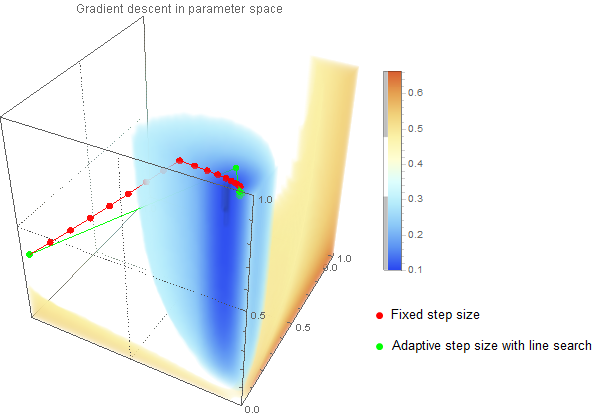
\includegraphics[width=1\linewidth]{images/nucleon_strong_red_parameterspace_path}
	\end{minipage}
	\caption[The steps of gradient descent methods with fixed step size and adaptive step size are shown in the parameter space]{The steps of gradient descent methods with fixed step size and adaptive step size are shown in the parameter space in Figure~\ref{fig:nucleon_parameterspace} (the step size is 0.1)}
	\label{fig:nucleon_parameterspace_path}
\end{figure}

\subsubsection{Parallel Line Search}
The classical gradient descent is a sequential algorithm. In its iterative procedure, the next iteration takes the result from the previous iteration as input.
However, the line search at each iteration can be computed in parallel to accelerate the optimization. This idea is particularly useful in our transfer function optimization, because the most expensive computation in our transfer function optimization is the evaluation of visibility-weighted saliency, which is required in the evaluation of the objective function at each iteration.

In this subsection, we propose a parallel line search strategy, which evaluates the objective function at different candidate points in parallel along the line search direction. With this parallel approach, the computing power of modern multi-core processors can be better exploited to accelerate the transfer function optimization. Specifically, parallel line search launches multiple threads to perform the line search. Each thread computes the visibility-weighted saliency and the objective function at a candidate point. Subsequently, the results at all the candidate points are aggregated and the candidate point with the minimum objective function value is chosen as the next step.

The parallel line search is shown as follows.

\begin{enumerate}
	\item Generate a list of step sizes $ S= \{ \gamma_{0},\gamma_{1},...,\gamma_{n-1} \} $ where $ \gamma_{i}=2^{i} $
	\item Evaluate $ f(x_{k}+\gamma_{i} g_{k}) $ in parallel for each $ \gamma_{i} $ in $ S $
	\item Find the index $ i $ of the minimum $ f(x_{k}+\gamma_{i} g_{k}) $, then $ \gamma_{i} $ is the chosen step size.
\end{enumerate}

The mechanism of the parallel line search is sightly different from the sequential line search. In the sequential line search, if the current candidate point does not meet the condition, the line search is terminated and the next candidate point would not be evaluated. By contrast, the parallel line search would always evaluate all the candidate points and pick the one with least value of the objective function. However, these two methods would have the same behavior if the objective function is a convex function.

The parallel line search strategy would introduce extra overhead of starting and terminating threads. Moreover, the number of threads should not exceed the number of cores of the processor, otherwise multiple threads have to share the same core and this would cause performance impact. The parallel line search is beneficial only when the evaluation of the objective function is more expensive than the parallel overhead.
In our case, the evaluation of the objective function is very computationally expensive. It requires computing the visibility fields, which in turn requires that a pass of slice-based volume rendering is performed.

Figure~\ref{fig:nucleon_naive_tooth_naive_rms_linesearch} displays results of applying the two line search methods in optimizing transfer functions. The two curves of objective functions are mostly overlapping, which indicates the two methods acts almost the same in choosing step sizes.

\begin{figure}
	\centering
	\begin{minipage}{.49\textwidth}
		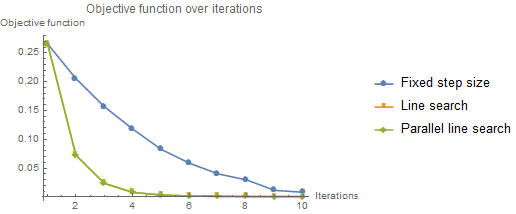
\includegraphics[width=1\linewidth]{images/nucleon_naive_rms_fixed_linesearch_parallel}
		\subcaption{}
	\end{minipage}~
	\begin{minipage}{.49\textwidth}
		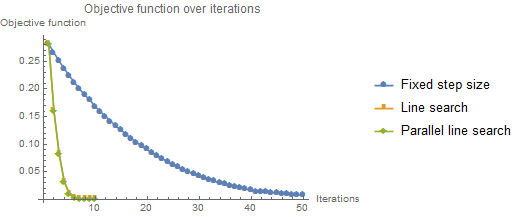
\includegraphics[width=1\linewidth]{images/tooth_naive_rms_fixed_linesearch_parallel}
		\subcaption{}
	\end{minipage}
	\caption[The line search and parallel line search are applied to transfer function optimization on the nuclon data set and the tooth data set respectively.]{The line search and parallel line search are applied to transfer function optimization on the nuclon data set (a) and the tooth data set (b) respectively. The two methods both converge ($F<0.03$) at step 4 for the nucleon data set and both converge at step 5 for the tooth data set. The two line search methods made very similar choices in step sizes.}
	\label{fig:nucleon_naive_tooth_naive_rms_linesearch}
\end{figure}

%-------------------------------------------------------------------------
\section{Results and Discussions}
In this section, we present some results to demonstrate the effectiveness of our approach on the nucleon data set ($ 41 \times 41 \times 41 $), a tooth data set ($ 140 \times 120 \times 161 $), a CT-knee (379 $ \times $ 229 $ \times $ 305) data set \cite{website:Roettger_volume_2013} and one time-step of a simulated turbulent vortex flow (128 $\times$ 128 $\times$ 128, 100 time-steps) \cite{website:Ma_repository_2013}.
%and four volumes of a horse embryo data set, which are the horse embryo at 35, 37, 39 and 42 days.
Results were obtained in our experimental programs written in Wolfram Mathematica 11 on a computer equipped with an Intel Xeon E3-1246 v3 processor, 16GB of RAM and a NVIDIA Quadro K4200 graphics card.
%Tests were performed on a computer equipped with an Intel Core i5-2410M CPU, 8GB of RAM and a NVIDIA GeForce GT 540M graphics card.

In the results, we display the transfer functions and volume rendered images before and after transfer function optimization, as well as the evolution of visibility-weighted saliency and opacity values of features during the iterations.
The feature visibility histograms \cite{wang_efficient_2011} are displayed along with the visibility-weighted saliency histograms for comparison.
0.05 is used as the step size and the objective function $ F $ falling below 0.03 is regarded as convergence.
The two optimization methods shown in the results are gradient descent with fixed step size and gradient descent with parallel line search, both using the Method 1 discussed in Section~\ref{estimating_descent_directions} for estimating descent directions.

Figure~\ref{fig:nucleon_naive_optimized} shows the optimization results of Figure~\ref{fig:nucleon_naive}. In Figure~\ref{fig:nucleon_naive_optimized} (a), the three features from outside to inside appear in different transparency levels, from weak to strong. This reveals a clear perspective of the three structures.
Figure~\ref{fig:nucleon_naive_optimized} (b) to (d) are the optimized transfer function, the feature visibility histogram and the visibility-weighted saliency histogram respectively.
Figure~\ref{fig:nucleon_naive_optimized} (e) and (f) are the evolution of visibility-weighted saliency of each feature over 10 iterations, in the gradient descent with fixed step sizes and adaptive step sizes using the parallel line search respectively. Figure~\ref{fig:nucleon_naive_optimized} (g) and (h) show scatter plots of visibility-weighted saliency and opacity in the iteration steps, with lines connecting adjacent steps.
The evolutions of the objective function are also shown in Figure~\ref{fig:nucleon_naive_tooth_naive_rms} (a) and Figure~\ref{fig:nucleon_naive_tooth_naive_rms_linesearch} (a) respectively.

Figure~\ref{fig:tooth_naive_optimized} (a), (c) and (d) display volume rendered images of the tooth data set before transfer function optimization. Figure~\ref{fig:tooth_naive_optimized} (b), (e) and (f) shows the same data sets after transfer function optimization.
Figure~\ref{fig:tooth_naive_optimized} (g) and (h) are the evolution of visibility-weighted saliency of each feature, over 50 iterations in the gradient descent with fixed step sizes, and over 10 iterations in adaptive step sizes using the parallel line search respectively. Figure~\ref{fig:tooth_naive_optimized} (i) and (j) illustrate the relationship between the visibility-weighted saliency and opacity of features, in the iterations of the two gradient descent methods respectively.
The evolutions of the objective function are also shown in Figure~\ref{fig:nucleon_naive_tooth_naive_rms} (b) and Figure~\ref{fig:nucleon_naive_tooth_naive_rms_linesearch} (b).

Figure~\ref{fig:CT-Knee_naive_optimized} shows the volume rendered images of a CT-Knee data set ((a) and (b)), and the feature visibility histograms and the visibility-weighted saliency histograms ((c) to (f)) before and after optimization respectively.

Figure~\ref{fig:vortex_naive_optimized} shows the volume rendered images of the first time-step of a vortex data set ((a) and (b)), and the feature visibility histograms and the visibility-weighted saliency histograms ((c) to (f)) before and after optimization respectively.

The evolution of visibility-weighted saliency of each feature and the relationship between the visibility-weighted saliency and opacity of features, in the iterations of the two gradient descent methods are displayed in Figure~\ref{fig:CT-Knee_naive_optimized} (g) to (j) and Figure~\ref{fig:vortex_naive_optimized} (g) to (j) for the CT-Knee data set and the vortex data set respectively.

In the optimized results of these 4 data sets, the visibility-weighted saliency values of the 3 features are very close to the user-specified targets, as shown in Figure~\ref{fig:nucleon_naive_optimized} (d), Figure~\ref{fig:tooth_naive_optimized} (f), and Figure~\ref{fig:CT-Knee_naive_optimized} (f).

Figure~\ref{fig:CT-Knee_naive_vortex_naive_rms_linesearch} displays the evolution of the objective function in the optimization of the CT-Knee data set and the vortex data set.
We noticed the two line search methods require much fewer steps to converge than the fixed step-size method and they made the same choices of adaptive step sizes during the iterations (the two curves completely overlapped).
Although the two line search methods use the same numbers of steps, our parallel line search method only took about half the time of the sequential line search method (Table~\ref{table:performance_table}).

Figure~\ref{fig:parallelsearch_performance} shows the convergence time of the parallel line search approach on the 4 data sets over 1, 2, 4 and 8 CPU threads respectively.
We observed that the computation time decreased as the number of threads increased. However, the speedup from 4 threads to 8 threads is minor, which may due to the fact that the CPU of the experiment computer only has 4 cores.

For the sake of clarity of presentation and convenience of the user study, the results in this section are includes cases of transfer functions with three features and three distinctive feature colors. See Appendix~\ref{Generality_of_TF} for details of applying the transfer function optimization approach to other transfer functions and other color schemes.

%\begin{table}[h]
%	\begin{tabular}{ c | l | l c r }
%		& & Fixed step size & Line search & Parallel line search \\
%		\hline
%		nucleon & Steps to converge & 37 & 4 & 4 \\
%		& Time (seconds) & 1.91 & 0.83 & 0.55 \\
%		\hline
%		tooth & Steps to converge & 47 & 4 & 4 \\
%		& Time (seconds) & 18.05 & 6.59 & 3.31 \\
%		\hline
%		CT-Knee & Steps to converge & 47 & 6 & 6 \\
%		& Time (seconds) & 120.38 & 59.01 & 33.41 \\
%		\hline
%		vortex & Steps to converge & 56 & 21 & 21 \\
%		& Time (seconds) & 24.95 & 25.42 & 14.92 \\
%	\end{tabular}
%	\caption[Performance of the 3 optimization approaches on the 4 volume data sets]{Performance of the 3 optimization approaches on the 4 volume data sets. ($ F<0.01 $ is regarded as convergence.)}
%	\label{table:performance_table}
%\end{table}

\begin{table}[h]
	\begin{tabular}{ c | l | l c r }
		& & Fixed step size & Line search & Parallel line search \\
		\hline
		nucleon & Steps to converge & 17 & 2 & 2 \\
		& Time (seconds) & 1.07 & 0.59 & 0.38 \\
		\hline
		tooth & Steps to converge & 21 & 2 & 2 \\
		& Time (seconds) & 7.56 & 3.25 & 1.57 \\
		\hline
		CT-Knee & Steps to converge & 17 & 2 & 2 \\
		& Time (seconds) & 33.84 & 17.81 & 9.26 \\
		\hline
		vortex & Steps to converge & 33 & 13 & 13 \\
		& Time (seconds) & 14.00 & 15.22 & 8.40 \\
	\end{tabular}
	\caption[Performance of the 3 optimization approaches]{Performance of the 3 optimization approaches showing steps and time (seconds) taken to converge ($ F<0.03 $ is regarded as convergence.)}
	\label{table:performance_table}
\end{table}


\subsubsection{Transfer Function Optimization For Time-Varying Data Sets}
Similar to the approach discussed in Section~\ref{adaptive_transfer_functions_for_time-varying_data_sets}, we apply our transfer function optimization on all the time steps of the vortex data set. Our optimizer dynamically optimizes the transfer function to the same user-specified target (equal weights i.e. (1/3, 1/3, 1/3) were set as target in this test) for each time step of the time-varying data set. 

Figure~\ref{fig:vorts_static} displays the temporal curves of the visibility-weighted saliency (VWS) and 2D feature saliency (2DFS, discussed in Section~\ref{2d_feature_saliency}) of the visualization with a static transfer function (optimized for the first time step) respectively.
Similarly, Figure~\ref{fig:vorts_dynamic} displays the temporal curves of the VWS and 2DFS of the visualization with a dynamic transfer function (optimized for each time step) respectively.
The VWS curves in Figure~\ref{fig:vorts_dynamic} (a) are more converged than the VWS curves in Figure~\ref{fig:vorts_static} (a) because the dynamic transfer function is constantly optimized towards the target (1/3, 1/3, 1/3).

The 2DFS curves in Figure~\ref{fig:vorts_static} (b) and Figure~\ref{fig:vorts_dynamic} (b) are provided as comparison for the fact that 2DFS is an image space technique independent from VWS. We notice that there are more small changes in the 2DFS curves in Figure~\ref{fig:vorts_static} (b) and the three curves (representing the 2DFS of the three features) cross each other more often than the 2DFS curves in Figure~\ref{fig:vorts_static} (b).

Time step 30 and 80 rendered with the static transfer function and the dynamic transfer function are displayed in Figure~\ref{fig:vorts_50_80_static} and Figure~\ref{fig:vorts_50_80_dynamic} respectively. As coherence can be an important factor in time-varying visualization, we notice the dynamic transfer function can maintain similar level of visual saliency for the purple feature when the sizes and proportions of the features change over time.

%Objective function
%Figure~\ref{fig:nucleon_strong_red_rms}

%Visibility-weighted saliency of each feature
%Figure~\ref{fig:nucleon_strong_red_saliency}
%
%Opacity of each feature
%Figure~\ref{fig:nucleon_strong_red_opacity}

%Before optimization
%Figure~\ref{fig:nucleon_strong_red}
%
%After optimization
%Figure~\ref{fig:nucleon_strong_red_optimized}

%\begin{figure}
%	\centering
%	\begin{minipage}{.35\textwidth}
%		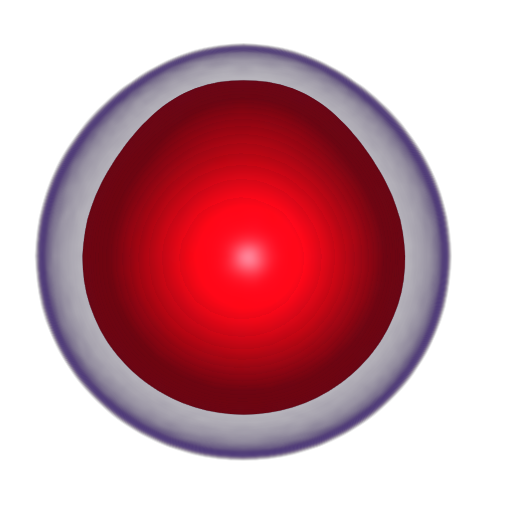
\includegraphics[width=1\linewidth]{images/nucleon_strong_red}
%	\end{minipage}~
%	\begin{minipage}{.2\textwidth}
%		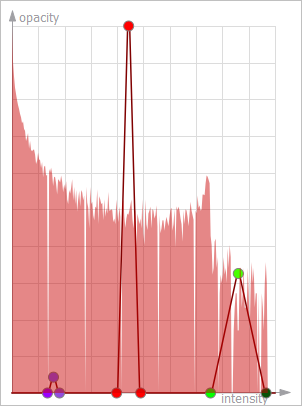
\includegraphics[width=1\linewidth]{images/tf_nucleon_strong_red}	
%	\end{minipage}~
%	\begin{minipage}{.4\textwidth}
%		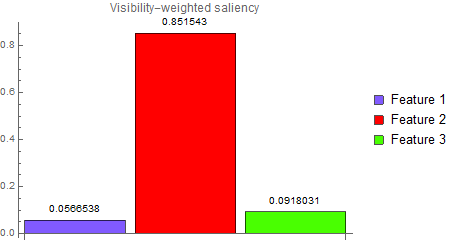
\includegraphics[width=1\linewidth]{images/nucleon_strong_red_visibility_saliency_weighted_chart}
%	\end{minipage}
%	\caption{Before optimization, the transfer function strongly emphasizes the red feature, which occludes the green feature inside. (Left: the volume rendered image of the nucleon data set; Middle: the transfer function; Right: the visibility-weighted saliency histogram)}
%	\label{fig:nucleon_strong_red}
%\end{figure}

\begin{figure}
	\centering
	\begin{minipage}{.3\textwidth}
		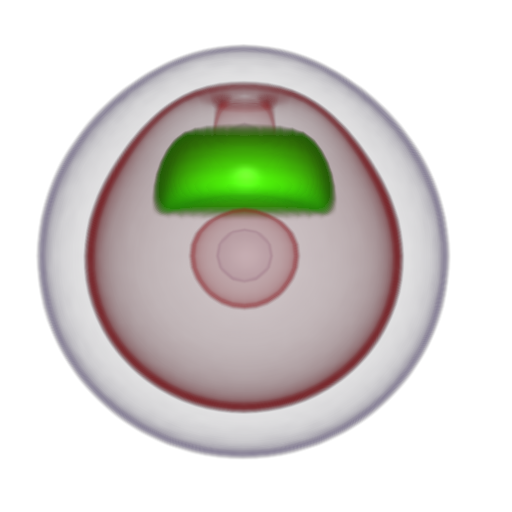
\includegraphics[width=1\linewidth]{images/nucleon_naive_optimized_linesearch}
		\subcaption{}
	\end{minipage}~
	\begin{minipage}{.15\textwidth}
		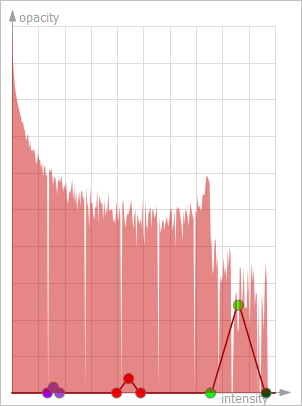
\includegraphics[width=1\linewidth]{images/tf_nucleon_naive_optimized_linesearch}
		\subcaption{}
	\end{minipage}~
	\begin{minipage}{.25\textwidth}
		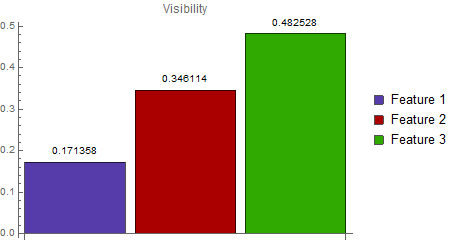
\includegraphics[width=1\linewidth]{images/nucleon_naive_optimized_linesearch_visibility_chart}
		\subcaption{}
	\end{minipage}~
	\begin{minipage}{.25\textwidth}
		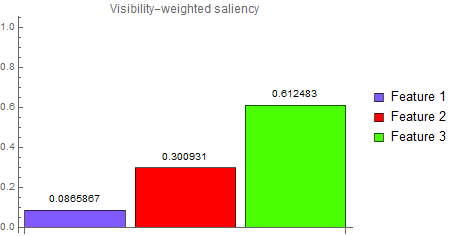
\includegraphics[width=1\linewidth]{images/nucleon_naive_optimized_linesearch_visibility_saliency_weighted_chart}
		\subcaption{}
	\end{minipage}
	
	\begin{minipage}{.49\textwidth}
		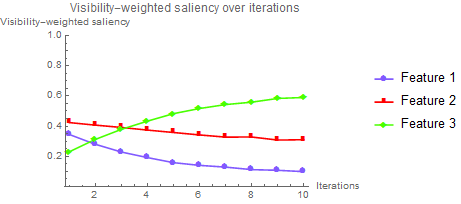
\includegraphics[width=1\linewidth]{images/nucleon_naive_saliency_fixed}
		\subcaption{}
	\end{minipage}~
	\begin{minipage}{.49\textwidth}
		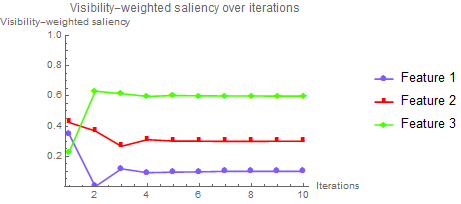
\includegraphics[width=1\linewidth]{images/nucleon_naive_saliency_parallelsearch}
		\subcaption{}
	\end{minipage}
	
	\begin{minipage}{.49\textwidth}
		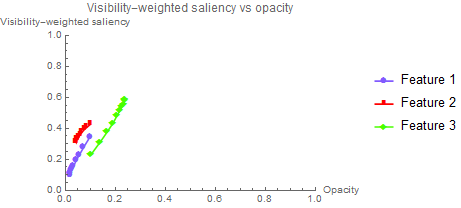
\includegraphics[width=1\linewidth]{images/nucleon_naive_saliencyopacity_fixed}
		\subcaption{}
	\end{minipage}~
	\begin{minipage}{.49\textwidth}
		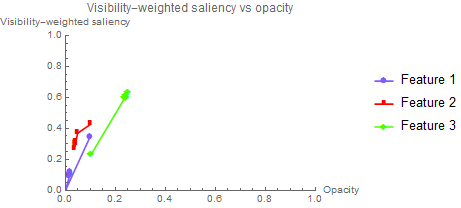
\includegraphics[width=1\linewidth]{images/nucleon_naive_saliencyopacity_parallelsearch}
		\subcaption{}
	\end{minipage}
	\caption[After optimization to target \{0.1, 0.3, 0.6\}, all the 3 features are visible and the green feature inside is particularly emphasized.]{After optimization to target \{0.1, 0.3, 0.6\}, all the 3 features are visible and the green feature inside is particularly emphasized. (a) The optimized volume rendered image of the nucleon data set; (b) The optimized transfer function; (c) The feature visibility histogram \cite{wang_efficient_2011}; (d) The visibility-weighted saliency histogram); (e) \& (g) Gradient descent with fixed step sizes; (f) \& (h) Gradient descent with parallel line search}
	\label{fig:nucleon_naive_optimized}
\end{figure}

\begin{figure}
	\centering
	\begin{minipage}{.4\textwidth}
		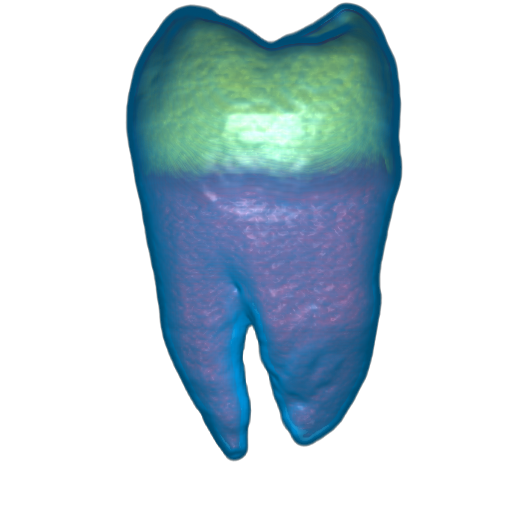
\includegraphics[width=1\linewidth]{images/tooth_naive}
		\subcaption{}
	\end{minipage}~
	\begin{minipage}{.4\textwidth}
		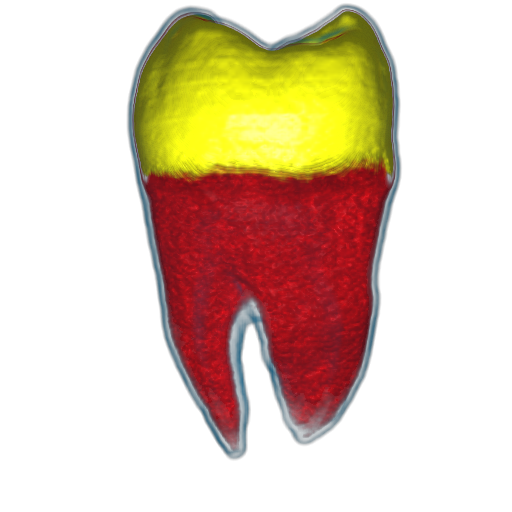
\includegraphics[width=1\linewidth]{images/tooth_naive_optimized_linesearch}
		\subcaption{}
	\end{minipage}
	
	\begin{minipage}{.24\textwidth}
		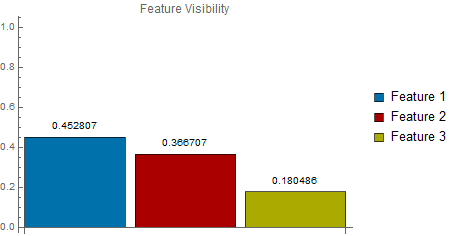
\includegraphics[width=1\linewidth]{images/tooth_naive_visibility_chart}
		\subcaption{}
	\end{minipage}~
	\begin{minipage}{.24\textwidth}
		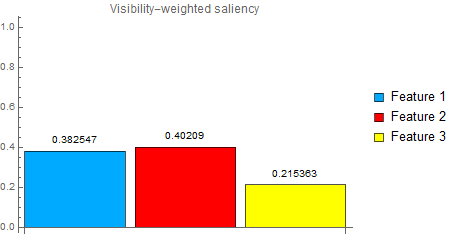
\includegraphics[width=1\linewidth]{images/tooth_naive_visibility_saliency_weighted_chart}
		\subcaption{}
	\end{minipage}~
	\begin{minipage}{.24\textwidth}
		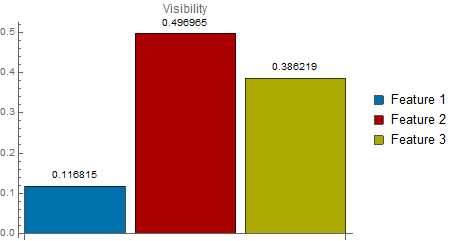
\includegraphics[width=1\linewidth]{images/tooth_naive_optimized_linesearch_visibility_chart}
		\subcaption{}
	\end{minipage}~
	\begin{minipage}{.24\textwidth}
		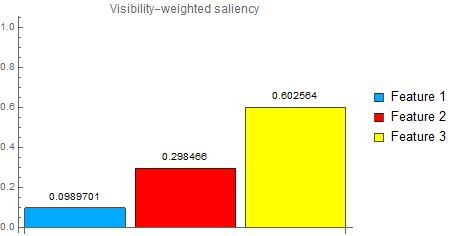
\includegraphics[width=1\linewidth]{images/tooth_naive_optimized_linesearch_visibility_saliency_weighted_chart}
		\subcaption{}
	\end{minipage}
	
	\begin{minipage}{.49\textwidth}
		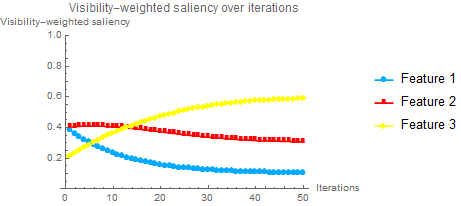
\includegraphics[width=1\linewidth]{images/tooth_naive_saliency_fixed}
		\subcaption{}
	\end{minipage}~
	\begin{minipage}{.49\textwidth}
		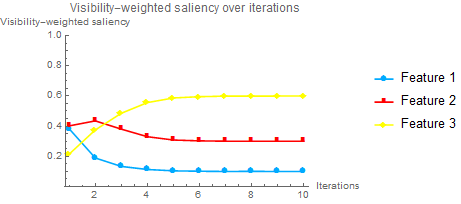
\includegraphics[width=1\linewidth]{images/tooth_naive_saliency_parallelsearch}
		\subcaption{}
	\end{minipage}
	
	\begin{minipage}{.49\textwidth}
		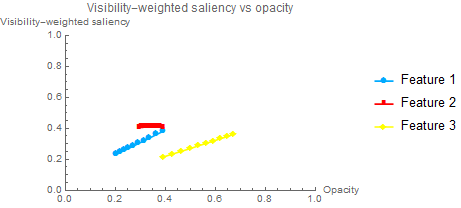
\includegraphics[width=1\linewidth]{images/tooth_naive_saliencyopacity_fixed}
		\subcaption{}
	\end{minipage}~
	\begin{minipage}{.49\textwidth}
		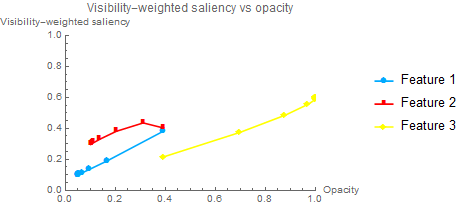
\includegraphics[width=1\linewidth]{images/tooth_naive_saliencyopacity_parallelsearch}
		\subcaption{}
	\end{minipage}
	\caption[After optimization to target \{0.1, 0.3, 0.6\}, all the 3 features are visible and the yellow feature inside is particularly emphasized.]{After optimization to target \{0.1, 0.3, 0.6\}, all the 3 features are visible and the yellow feature inside is particularly emphasized. (g) \& (i) Gradient descent with fixed step sizes; (h) \& (j) Gradient descent with parallel line search}
	\label{fig:tooth_naive_optimized}
\end{figure}

\begin{figure}
	\centering
	\begin{minipage}{.4\textwidth}
		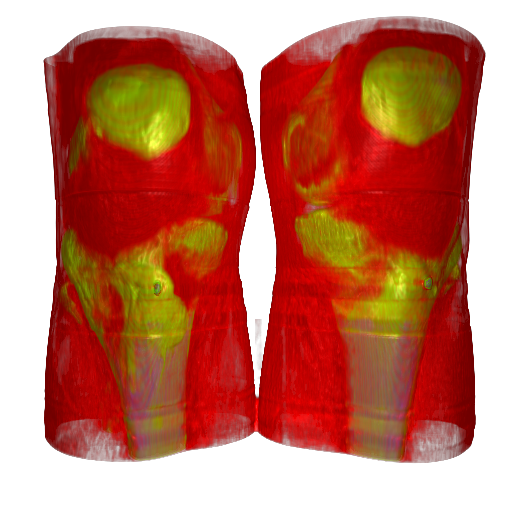
\includegraphics[width=1\linewidth]{images/CT-Knee_naive}
		\subcaption{}
	\end{minipage}~
	\begin{minipage}{.4\textwidth}
		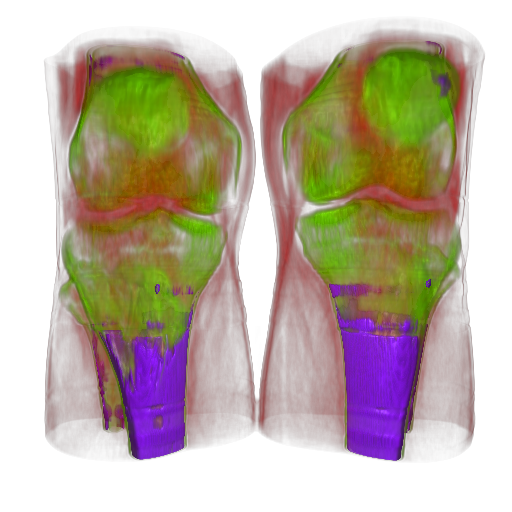
\includegraphics[width=1\linewidth]{images/CT-Knee_naive_optimized_linesearch}
		\subcaption{}
	\end{minipage}
	
	\begin{minipage}{.24\textwidth}
		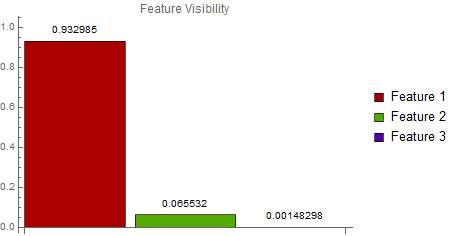
\includegraphics[width=1\linewidth]{images/CT-Knee_naive_visibility_chart}
		\subcaption{}
	\end{minipage}~
	\begin{minipage}{.24\textwidth}
		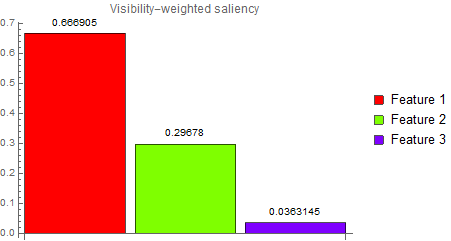
\includegraphics[width=1\linewidth]{images/CT-Knee_naive_visibility_saliency_weighted_chart}
		\subcaption{}
	\end{minipage}~
	\begin{minipage}{.24\textwidth}
		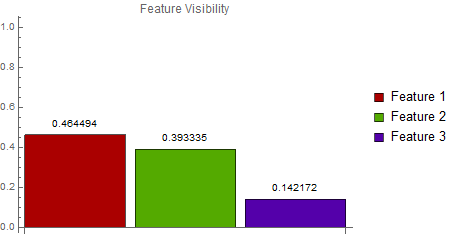
\includegraphics[width=1\linewidth]{images/CT-Knee_naive_optimized_linesearch_visibility_chart}
		\subcaption{}
	\end{minipage}~
	\begin{minipage}{.24\textwidth}
		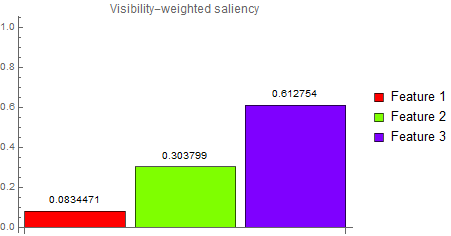
\includegraphics[width=1\linewidth]{images/CT-Knee_naive_optimized_linesearch_visibility_saliency_weighted_chart}
		\subcaption{}
	\end{minipage}	
	
	\begin{minipage}{.49\textwidth}
		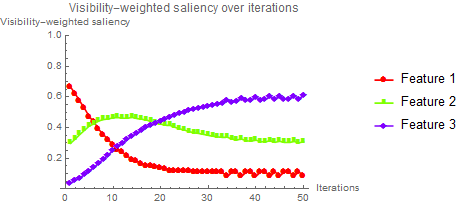
\includegraphics[width=1\linewidth]{images/CT-Knee_naive_saliency_fixed}
		\subcaption{}
	\end{minipage}~
	\begin{minipage}{.49\textwidth}
		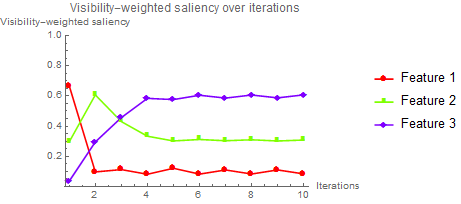
\includegraphics[width=1\linewidth]{images/CT-Knee_naive_saliency_parallelsearch}
		\subcaption{}
	\end{minipage}
	
	\begin{minipage}{.49\textwidth}
		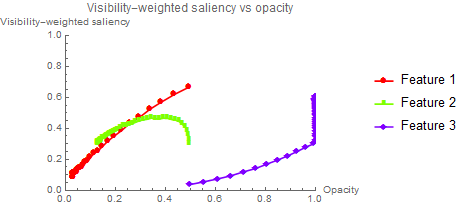
\includegraphics[width=1\linewidth]{images/CT-Knee_naive_saliencyopacity_fixed}
		\subcaption{}
	\end{minipage}~
	\begin{minipage}{.49\textwidth}
		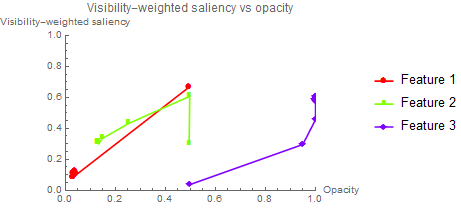
\includegraphics[width=1\linewidth]{images/CT-Knee_naive_saliencyopacity_parallelsearch}
		\subcaption{}
	\end{minipage}
	\caption[After optimization to target \{0.1, 0.3, 0.6\}, all the 3 features are visible, and the green and the purple features inside become clearer.]{After optimization to target \{0.1, 0.3, 0.6\}, all the 3 features are visible, and the green and the purple features inside become clearer. (g) \& (i) Gradient descent with fixed step sizes; (h) \& (j) Gradient descent with parallel line search}
	\label{fig:CT-Knee_naive_optimized}
\end{figure}

\begin{figure}
	\centering
	\begin{minipage}{.4\textwidth}
		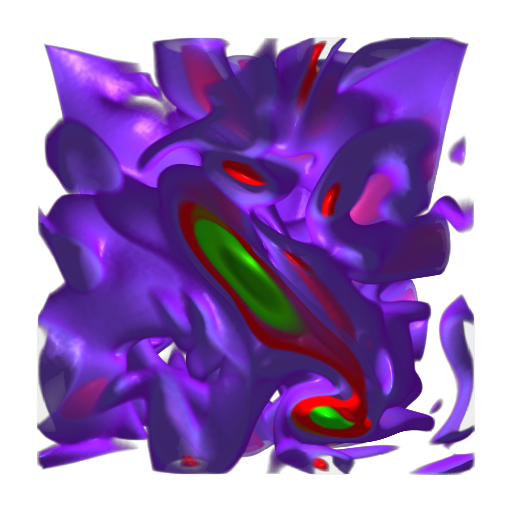
\includegraphics[width=1\linewidth]{images/vortex_naive}
		\subcaption{}
	\end{minipage}~
	\begin{minipage}{.4\textwidth}
		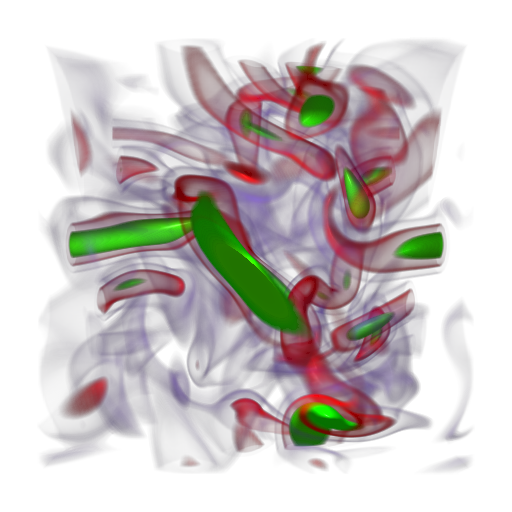
\includegraphics[width=1\linewidth]{images/vortex_naive_optimized_fixed}
		\subcaption{}
	\end{minipage}

	\begin{minipage}{.24\textwidth}
		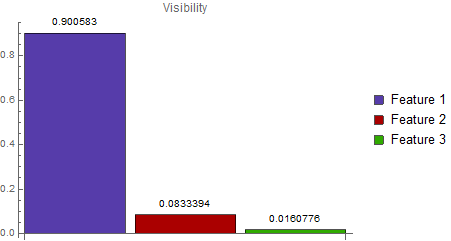
\includegraphics[width=1\linewidth]{images/vortex_naive_visibility_chart}
		\subcaption{}
	\end{minipage}~
	\begin{minipage}{.24\textwidth}
		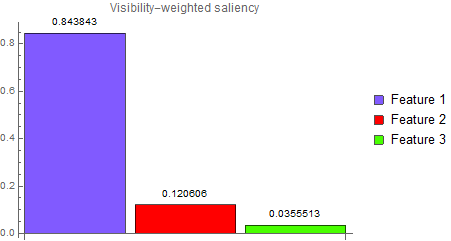
\includegraphics[width=1\linewidth]{images/vortex_naive_visibility_saliency_weighted_chart}
		\subcaption{}
	\end{minipage}~
	\begin{minipage}{.24\textwidth}
		\includegraphics[width=1\linewidth]{images/vortex_naive_optimized_fixed_visibility_chart}
		\subcaption{}
	\end{minipage}~
	\begin{minipage}{.24\textwidth}
		\includegraphics[width=1\linewidth]{images/vortex_naive_optimized_fixed_visibility_saliency_weighted_chart}
		\subcaption{}
	\end{minipage}	
	
	\begin{minipage}{.49\textwidth}
		\includegraphics[width=1\linewidth]{images/vortex_naive_saliency_fixed}
		\subcaption{}
	\end{minipage}
	\begin{minipage}{.49\textwidth}
		\includegraphics[width=1\linewidth]{images/vortex_naive_saliency_parallelsearch}
		\subcaption{}
	\end{minipage}
	
	\begin{minipage}{.49\textwidth}
		\includegraphics[width=1\linewidth]{images/vortex_naive_saliencyopacity_fixed}
		\subcaption{}
	\end{minipage}~
	\begin{minipage}{.49\textwidth}
		\includegraphics[width=1\linewidth]{images/vortex_naive_saliencyopacity_parallelsearch}
		\subcaption{}
	\end{minipage}
	\caption[After optimization to target \{1/3, 1/3, 1/3\}, all the 3 features are visible and the green feature inside is particularly more emphasized in comparison to the unoptimized result.]{After optimization to target \{1/3, 1/3, 1/3\}, all the 3 features are visible and the green feature inside is particularly more emphasized in comparison to the unoptimized result. (g) \& (i) Gradient descent with fixed step sizes; (h) \& (j) Gradient descent with parallel line search}
	\label{fig:vortex_naive_optimized}
\end{figure}

\begin{figure}
	\centering
	\begin{minipage}{.49\textwidth}
		\includegraphics[width=1\linewidth]{images/CT-Knee_naive_rms_fixed_linesearch_parallel}
		\subcaption{}
	\end{minipage}~
	\begin{minipage}{.49\textwidth}
		\includegraphics[width=1\linewidth]{images/vortex_naive_rms_fixed_linesearch_parallel}
		\subcaption{}
	\end{minipage}
	\caption[The line search and parallel line search are applied to transfer function optimization on the CT-Knee data set and the first time step of the vortex data set respectively.]{The line search and parallel line search are applied to transfer function optimization on the CT-Knee data set (a) and the first time step of the vortex data set (b) respectively. The two methods both converge ($F<0.03$) at step 4 for the nucleon data set and both converge at step 5 for the tooth data set. The two line search methods made very similar choices in step sizes.}
	\label{fig:CT-Knee_naive_vortex_naive_rms_linesearch}
\end{figure}

\begin{figure}
	\centering
	\begin{minipage}{.49\textwidth}
		\includegraphics[width=1\linewidth]{nucleon_performance}
		\subcaption{nucleon}
	\end{minipage}~
	\begin{minipage}{.49\textwidth}
		\includegraphics[width=1\linewidth]{tooth_performance}
		\subcaption{tooth}
	\end{minipage}
	\begin{minipage}{.49\textwidth}
		\includegraphics[width=1\linewidth]{CT-Knee_performance}
		\subcaption{CT-Knee}
	\end{minipage}~
	\begin{minipage}{.49\textwidth}
		\includegraphics[width=1\linewidth]{vortex_performance}
		\subcaption{vortex}
	\end{minipage}
	\caption[Performance of parallel line search]{Performance of parallel line search (seconds taken to converge) over different number of CPU threads}
	\label{fig:parallelsearch_performance}
\end{figure}

\begin{figure}
	\centering
	\begin{minipage}{.49\textwidth}
		\includegraphics[width=1\linewidth]{images/vorts_static_VWS}
		\subcaption{}
	\end{minipage}~
	\begin{minipage}{.49\textwidth}
		\includegraphics[width=1\linewidth]{images/vorts_static_2DFS}
		\subcaption{}
	\end{minipage}
	\caption{(a) VWS and (b) 2DFS of the vortex data set with a static transfer function only optimized for the first time step}
	\label{fig:vorts_static}
\end{figure}

\begin{figure}
	\centering
	\begin{minipage}{.49\textwidth}
		\includegraphics[width=1\linewidth]{images/vorts_optimized_parallelsearch_VWS}
		\subcaption{}
	\end{minipage}~
	\begin{minipage}{.49\textwidth}
		\includegraphics[width=1\linewidth]{images/vorts_optimized_parallelsearch_2DFS}
		\subcaption{}
	\end{minipage}
	\caption{(a) VWS and (b) 2DFS of the vortex data set with a dynamic transfer function optimized for each time step}
	\label{fig:vorts_dynamic}
\end{figure}

\begin{figure}
	\centering
	\begin{minipage}{.49\textwidth}
		\includegraphics[width=1\linewidth]{images/vorts30_static}
		\subcaption{}
	\end{minipage}~
	\begin{minipage}{.49\textwidth}
		\includegraphics[width=1\linewidth]{images/vorts80_static}
		\subcaption{}
	\end{minipage}
	\caption{Time step 30 (a) and time step 80 (b) rendered with a static transfer function only optimized for the first time step}
	\label{fig:vorts_50_80_static}
\end{figure}

\begin{figure}
	\centering
	\begin{minipage}{.49\textwidth}
		\includegraphics[width=1\linewidth]{images/vorts30_optimized_parallelsearch}
		\subcaption{}
	\end{minipage}~
	\begin{minipage}{.49\textwidth}
		\includegraphics[width=1\linewidth]{images/vorts80_optimized_parallelsearch}
		\subcaption{}
	\end{minipage}
	\caption{Time step 30 (a) and time step 80 (b) rendered with a dynamic transfer function optimized for each time step}
	\label{fig:vorts_50_80_dynamic}
\end{figure}

%\begin{table}[h]
%	\begin{tabular}{ l | l c r }
%		& Fixed step size & Line search & Parallel line search \\
%		\hline
%		Time (seconds) & 18.05 & 6.59 & 3.31 \\
%		\hline
%		Iterations to converge (at 0.01) & 47 & 4 & 4 \\
%	\end{tabular}
%	\caption[Table caption text]{Performance of the 3 optimization approaches on the tooth data set ($ 140 \times 120 \times 161 $)}
%	\label{table:tooth_table}
%\end{table}
%
%\begin{table}[h]
%	\begin{tabular}{ l | l c r }
%		& Fixed step size & Line search & Parallel line search \\
%		\hline
%		Time (seconds) & 120.38 & 59.01 & 33.41 \\
%		Iterations to converge (at 0.01) & 47 & 6 & 6 \\
%	\end{tabular}
%	\caption[Table caption text]{Performance of the 3 optimization approaches on the CT-Knee data set ($ 379 \times 229 \times 305 $)}
%	\label{table:CT-Knee_table}
%\end{table}
%
%\begin{table}[h]
%	\begin{tabular}{ l | l c r }
%		& Fixed step size & Line search & Parallel line search \\
%		\hline
%		Time (seconds) & 24.95 & 25.42 & 14.92 \\
%		Iterations to converge (at 0.01) & 56 & 21 & 21 \\
%	\end{tabular}
%	\caption[Table caption text]{Performance of the 3 optimization approaches on the vortex data set ($ 128 \times 128 \times 128 $)}
%	\label{table:vortex_table}
%\end{table}

%-------------------------------------------------------------------------
\section{Conclusions}
This chapter proposes a novel transfer function optimization approach using the visibility-weighted saliency metric.
With this approach, the design of transfer functions becomes more intuitive. This approach allows the user to directly set target visibility-weighted saliency for features of interest and then the transfer function is automatically refined to match the visibility-weighted saliency of the features with user-defined targets. In addition, a parallel line search strategy is presented for exploiting the computing power of multi-core processors to improve the performance of the transfer function optimization approach.
This approach has proven to be effective over several volume data sets.
%-------------------------------------------------------------------------
